\section{Электромагнитная индукция}
%TODO Черепанов катушка + конденсатор + перемычка

\begin{ex}
\hspace{0pt} \\
\begin{minipage}{.65\textwidth}
(1998) По двум вертикальным рейкам, соединенным внизу сопротивлением $R$ и вверху источником с ЭДС $\mathcal{E}$ и внутренним сопротивлением $r$, без трения скользит проводник $AC$, длина которого $L$, масса $m$. 
Система находится в однородном магнитном поле с индукцией $B$, направленной за рисунок. 
Найдите установившуюся скорость проводника в поле силы тяжести, пренебрегая трением и сопротивлением реек и проводника.
\end{minipage}
\begin{minipage}{.35\textwidth}
\centering
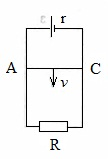
\includegraphics[width = 0.7 \textwidth]{121998EMIConductorAC.jpg}
\end{minipage}
\begin{ans}
$v = \frac{Rr}{lB(R+r)}\left( \frac{mg}{Bl} - \frac{\mathcal{E}}{r} \right)$
\end{ans}
\end{ex}

\begin{ex}
(2001) Две параллельные медные шины наклонены к горизонту под углом  $\alpha$. 
По ним скользит под действием силы тяжести медная перемычка массы $m$. Шины замкнуты катушкой с индуктивностью $L$. 
Система находится в однородном магнитном поле индукции $B$, перпендикулярном плоскости, в которой движется перемычка. 
Коэффициент трения перемычки о шины равен $\mu$. Каков будет характер движения перемычки? Сопротивлением шин, перемычки и катушки пренебречь.
\begin{ans}

\end{ans}
\end{ex}

\begin{ex}
(2004) Металлический стержень массы $m$ и длины $L$ подвешен горизонтально на двух легких проводах длиной $h$ в магнитном поле, 
индукция которого $B$ направлена вертикально вниз. К точкам крепления проводов подключен конденсатор емкостью $C$. 
Стержень вывели из положения равновесия и отпустили. Определить период малых колебаний стержня $T$. Сопротивлением стержня и проводов пренебречь.
\begin{ans}
$T = 2\pi \sqrt{\frac{l}{g} \left( 1 + \frac{B^2L^2C}{ml} \right)}$
\end{ans}
\end{ex}

%Ижевск
\begin{ex}
\hspace{0pt} \\
\begin{minipage}{.65\textwidth}
По двум параллельным металлическим направляющим, наклоненным под углом $\alpha$ к горизонту и 
расположенным на расстоянии $l$ друг от друга, может скользить без трения металлическая перемычка массой $m$. 
Направляющие замкнуты снизу на незаряженный конденсатор емкостью $C$, и вся конструкция находится в магнитном поле, индукция которого $B$ направлена по вертикали. В начальный момент перемычку удерживают на расстоянии $l$ от основания "горки". 
Определите время $t$, за которое перемычка достигнет основания "горки" после того, как ее отпустят. 
Омическим сопротивлением и индуктивностью контура пренебречь.
\end{minipage}
\begin{minipage}{.35\textwidth}
\centering
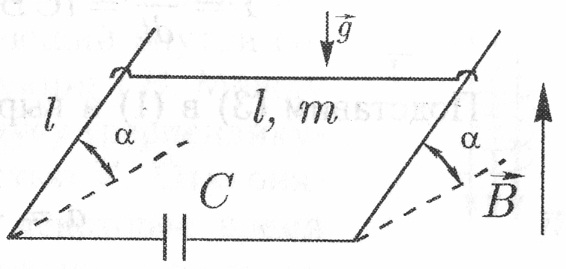
\includegraphics[width = 0.9 \textwidth]{1211EMIHillAndBridge.jpg}
\end{minipage}
\begin{ans}
$t=\sqrt{\frac{2l}{g \sin \alpha} \left( 1 + \frac{C l^2B^2 \cos^2 \alpha}{m} \right)}$
\end{ans}
\end{ex}

%Иродов-2.325
\begin{ex}
\hspace{0pt} \\
\begin{minipage}{.65\textwidth}
(2001) На расстоянии $a$ и $b$ от длинного прямого провода с током $I$ расположены два параллельных ему провода, 
замкнутые с одной стороны сопротивлением $R$. По проводам без трения перемещаются с постоянной скоростью $v$ стержень-перемычку. 
Пренебрегая сопротивлением проводов, стержня и контактов, найдите силу, необходимую для поддержания постоянства скорости. 
На каком расстоянии от ближнего провода нужно приложить силу, чтобы избежать вращения стержня?
\end{minipage}
\begin{minipage}{.35\textwidth}
\centering
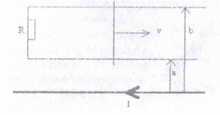
\includegraphics[width = 0.9 \textwidth]{122001EMIWiresAndBar.jpg}
\end{minipage}
\begin{ans}
$F=\frac{\mu_0^2 I^2 v}{4 \pi^2 R} \log^2 \frac{b}{a}$
\end{ans}
\end{ex}

%Ижевск
\begin{ex}
\hspace{0pt} \\
\begin{minipage}{.65\textwidth}
(2002) Прямоугольная рамка со сторонами $a$ и $b$ находится в одной плоскости с прямым проводником, по которому течет ток $I$, на расстоянии $L$ от него. Какой импульс получит рамка при выключении тока в проводе, если активное сопротивление рамки равно $R$, а реактивным сопротивлением ее можно пренебречь? 
Считать, что за время передачи импульса рамка заметно не перемещается.
\end{minipage}
\begin{minipage}{.35\textwidth}
\centering
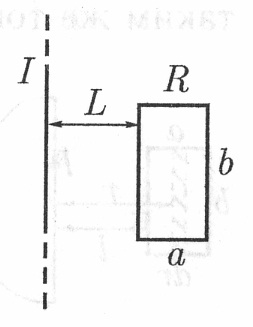
\includegraphics[width = 0.9 \textwidth]{122002EMIFrame.jpg}
\end{minipage}
\begin{ans}
$p=\frac{\mu_0^2ab^2I^2}{8\pi^2RL(L+a)}\log\left( 1+\frac{a}{L} \right)$
\end{ans}
\end{ex}

% Московская олимпиада школьников
\begin{ex}
\hspace{0pt} \\
\begin{minipage}{.65\textwidth}
Параллельные рельсы длиной $2L$ закреплены на горизонтальной плоскости на расстоянии $l$ друг от друга. 
К их концам подсоединены две одинаковые батареи с ЭДС  $\mathcal{E}$. На рельсах лежит перемычка массы $m$, 
которая может поступательно скользить вдоль них. Вся система помещена в однородное вертикальное магнитное поле с индукцией $B$. 
Считая, что сопротивление перемычки равно $R$, а сопротивление единицы длины каждого из рельсов равно $\rho$, найдите период малых колебаний, возникающих при смещении перемычки от положения равновесия, пренебрегая затуханием, внутренним сопротивлением источников, сопротивлением контактов, а также индуктивностью цепи.
\end{minipage}
\begin{minipage}{.35\textwidth}
\centering
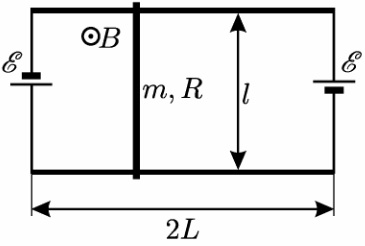
\includegraphics[width = 0.9 \textwidth]{1214EMIRailsAndBridge.jpg}
\end{minipage}
\begin{ans}
$T_0 = 2 \pi \sqrt{\frac{mL(\rho L + R)}{\mathcal{E}lB}}$
\end{ans}
\end{ex}

\begin{ex}
(2015) Проводящая квадратная рамка пересекает область однородного магнитного поля с шириной $d$, линии напряженности которого перпендикулярны плоскости рамки. При этом скорость рамки, равная $v_0$ до входа в магнитное поле уменьшается в 2 раза Масса рамки равна $m$, сопротивление рамки — $R$, величина вектора магнитной индукции - $B$. 1) Объясните, почему в рамке при пересечении магнитного поля выделяется тепло и найдите его. 2) Определите длину стороны рамки $a$ предполагая, что $a<d$. 3) Определите длину стороны рамки $a$ предполагая, что $a>d$.
\begin{ans}
1) $Q = 3mv_0^2/8$; 2) $a=\sqrt[3]{\frac{mv_0R}{4B^2}}$; 3) $a=\sqrt{\frac{mv_0R}{4B^2d}}$
\end{ans}
\end{ex}